\ofjob{Red Mage}
{
	\ofquote{"Oh, I’ll show you how lightning strikes."\\}{Lightning}\\\\
	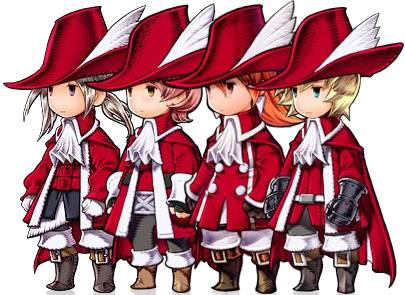
\includegraphics[width=\columnwidth]{./art/jobs/redmage.jpg}\ofrow
	\accf{Red Mages} are very versatile and possess a wide variety of abilities, but can also hold their own in melee combat. 
%	Although they excel in neither discipline, Red Mages are still a force to be reckoned with.
}
{Rod or Sword}{Light Armor or Robe}{
	Level 1: & HP~+20 & MP~+21 & AGI~+3 & STR +1 \\
	Level 2: & HP~+5  & MP~+10 & MAG~+1 & DEF~+1 \\
	Level 3: & \multicolumn{3}{l}{Archetype Attribute Bonus}   \\
	Level 4: & HP~+10 & MP~+5  & STR~+1 & RES~+1 \\   
	Level 5: & HP~+5  & MP~+10 & MAG~+2 & 		  \\ 
	Level 6: & HP~+5 & MP~+10  & STR~+1 &	MAG~+1 \\ 
	Level 7: & HP~+10  & MP~+10 & DEF~+1 \\ 
	Level 8: & HP~+10 & MP~+5  & STR~+1 & MAG~+1 \\ 
	Level 9: & HP~+5  & MP~+10 & RES~+2 \\ 
	Level 10: & HP~+10 & MP~+10 & STR~+1 		  
}{	
	\ofjobspell{Fire}{4}{0r}{Single}{3u}{You deal 2d fire damage to the target.}{\fire}{1}\ofabilitygap
	\ofjobspell{Blizzard}{4}{0r}{Single}{3u}{You deal 2d ice damage to the target.}{\ice}{1}\ofabilitygap
	\ofjobspell{Thunder}{4}{0r}{Single}{3u}{You deal 2d lightning damage to the target.}{\lightning}{1}\ofabilitygap
	\ofjobspell{Regen}{6}{0r}{Single}{5u}{The target gains Regen for 3 rounds.}{}{2}\ofabilitygap
	\ofjobspell{Blind}{6}{0r}{Single}{5u}{The target makes a DC~8 check and suffers Blind for 3 rounds upon failure.}{\blind}{4}\ofabilitygap	
	\ofjobspell{Vox}{6}{0r}{Single}{5u}{Remove one Status Effects except KO from the target. Also, the target becomes Immune to that Status Effect for 5 rounds.}{}{6}\ofabilitygap
	\ofjobspell{Imperil}{8}{0r}{Single}{5u}{The target suffers DeDEF and DeRES for 3 rounds.}{}{8}\ofabilitygap
	\ofjobspell{Wall}{8}{0r}{Single}{5u}{The target gains EnDEF and EnRES for 3 rounds.}{}{8}\ofabilitygap
	\ofjobspell{Dualcast}{2}{0r}{Single}{Self}{You begin casting two spells of your choice simultaneously, but need to spend the necessary MP for both.}{}{10}
}{
	\ofarchetypet{Ravager}
	{HP~+6 & MP~+14 & MAG~+2 & RES~+1}
	{\ofarchetypespella{Osmosis}{0}{0r}{Single}{5u}{You regain MP equal to your MAG and the target's MP is reduced by the same amount.}{}}
	{\ofarchetypepassive{Overwhelm}{When you inflict elemental damage, the target gains a weakness against that type until the end of your next turn. If he already has a Resilience against it, that is negated instead.}}
	{\ofarchetypereaction{Swiftcast}{Once per round, right after an enemy within 5u uses an action, you can immediately cast a spell on him.}}
	{\ofarchetypespellb{NulElement}{10}{0r}{Single}{5u}{Choose an element (e.g. fire). The target does not suffer any damage of the chosen element for 3 rounds.}{}}
}{
	\ofarchetypet{Spellblade}
	{HP~+14 & MP~+6 & STR~+2 & DEF~+1}
	{\ofarchetypetecha{Elemental Strike}{6}{0r}{Single}{Weapon}{Choose an element (e.g. fire) and make an Attack. If you hit, the damage is of magical type with the chosen element and you also add your MAG to the damage dealt.}{}}
	{\ofarchetypepassive{Magic Weapon}{Whenever you cast Magic, you can choose to store the spell inside your weapon. In this case, the spell's MP cost is halved. All stored spells take effect together with your next successful Attack and you can chose targets within their range including yourself. You cannot store more than two spells at once inside your weapon.}}
	{\ofarchetypereaction{Mana Shield}{Whenever your HP is reduced, you can instead choose to reduce your MP by the same amount.}}
	{\ofarchetypetechb{Magic Barrier}{10}{0r}{Single}{5u}{For the next 3 rounds, the target can evade the effect of spells and techs by passing an evasion check.}{}}
}